\documentclass[12pt]{article}


\usepackage{amssymb}
\usepackage{amsmath}
\usepackage{fullpage}
\usepackage{epsfig}
\usepackage{epstopdf, xcolor, hyperref}
\everymath{\displaystyle}
\usepackage{enumerate}



\begin{document}

\begin{center}
\underline{\LARGE{Parametric Equations of Lines}}
\end{center}

\noindent SUGGESTED REFERENCE MATERIAL:

\bigskip

\noindent As you work through the problems listed below, you should reference Chapter 11.5 of the recommended textbook (or the equivalent chapter in your alternative textbook/online resource) and your lecture notes.

\bigskip

\noindent EXPECTED SKILLS:

\begin{itemize}

\item Be able to find the parametric equations of a line that satisfies certain conditions by finding a point on the line and a vector parallel to the line. 

\item Know how to determine whether two lines in space are parallel, skew, or intersecting.  And, if the lines intersect, be able to determine the point of intersection.

\item Know how to determine where a line intersects a surface.

\end{itemize}

\noindent PRACTICE PROBLEMS:

\medskip

\noindent {\bf For problems 1-4, compute parametric equations of the line which satisfies the given conditions.}

\begin{enumerate}

\item The line which passes through the point $(1,0,-1)$  and is parallel to $\overrightarrow{v}=\langle 1,-2,0\rangle$.

\includegraphics[scale=0.5]{start.pdf}
{{$x=1+t, y=-2t, z=-1$}}
\includegraphics[scale=0.5]{end.pdf}


\item The line which passes through points $A(3,-6,6)$ and $B(2,0,7)$.

\includegraphics[scale=0.5]{start.pdf}
{{$x=3-t,y=-6+6t,z=6+t$}}
\includegraphics[scale=0.5]{end.pdf}


\item The line which passes through the point $(-1,2,4)$ and is parallel to $L_1=\left\{\begin{array}{l}
x=3-4t\\
y=3+2t\\
z=t\end{array}\right.$

\includegraphics[scale=0.5]{start.pdf}
{{$x=-1-4t,y=2+2t,z=4+t$}}
\includegraphics[scale=0.5]{end.pdf}


\item The line which passes through the point $(-2,1,4)$ and is parallel to both the $xy$-plane and the $xz$-plane.

\includegraphics[scale=0.5]{start.pdf}
{{$x=-2+t,y=1,z=4$; Detailed Solution: \textcolor{blue}{\href{http://www.math.drexel.edu/classes/Calculus/resources/Math200HW/Solutions/05_200_Lines_04.pdf}{Here}}}}
\includegraphics[scale=0.5]{end.pdf}


\item Is the line which passes through points $A_1(1,2,3)$ and $B_1(5,8,9)$ parallel to the line which passes through points $A_2(-2,5,3)$ and $B_2(4,14,12)$?

\includegraphics[scale=0.5]{start.pdf}
{{Yes.}}
\includegraphics[scale=0.5]{end.pdf}


\item Find the coordinates of the point at which the line $L_1=\left\{\begin{array}{l}
x=3-6t\\
y=3+3t\\
z=t\end{array}\right.$ intersects the given plane:

\begin{enumerate}

\item The $xy$-plane.

\includegraphics[scale=0.5]{start.pdf}
{{$(x,y,z)=(3,3,0)$}}
\includegraphics[scale=0.5]{end.pdf}


\item The $xz$-plane.

\includegraphics[scale=0.5]{start.pdf}
{{$(x,y,z)=(9,0,-1)$}}
\includegraphics[scale=0.5]{end.pdf}


\item The $yz$-plane.

\includegraphics[scale=0.5]{start.pdf}
{{$(x,y,z)=\left(0,\frac{9}{2},\frac{1}{2}\right)$}}
\includegraphics[scale=0.5]{end.pdf}


\end{enumerate}

\item Find the coordinates of the points in 3-space where the line $L_1=\left\{\begin{array}{l}
x=t\\y=1+t\\
z=1-t\end{array}\right.$ intersects the sphere $x^2+y^2+z^2=29$.

\includegraphics[scale=0.5]{start.pdf}
{{$(x,y,z)=(3,4,-2)$ and $(x,y,z)=(-3,-2,4)$; Detailed Solution: \textcolor{blue}{\href{http://www.math.drexel.edu/classes/Calculus/resources/Math200HW/Solutions/05_200_Lines_07.pdf}{Here}}}}
\includegraphics[scale=0.5]{end.pdf}


\end{enumerate}

\noindent{\bf For problems 8-11, determine whether the given lines intersect, are parallel, or are skew.  If the lines intersect, find the point of intersection.}

\begin{enumerate}
\setcounter{enumi}{7}

\item $L_1: x=2+3t, y=1-2t, z=4+5t$\\
$L_2: x=3-6t, y=-2+4t, z=-1-10t$

\includegraphics[scale=0.5]{start.pdf}
{{The lines are parallel.}}
\includegraphics[scale=0.5]{end.pdf}


\item $L_1: x=1, y=t, z=2-t$\\
$L_2: x=2+3t, y=4-3t, z=t$

\includegraphics[scale=0.5]{start.pdf}
{{The lines are skew.}}
\includegraphics[scale=0.5]{end.pdf}


\item $L_1: x=1-2t, y=14+t, z=5-t$\\
$L_2: x=t, y=4+3t, z=3+t$

\includegraphics[scale=0.5]{start.pdf}
{{The lines intersect at the point $(x,y,z)=(3,13,6)$; Detailed Solution: \textcolor{blue}{\href{http://www.math.drexel.edu/classes/Calculus/resources/Math200HW/Solutions/05_200_Lines_10.pdf}{Here}}}}
\includegraphics[scale=0.5]{end.pdf}


\item $L_1: x=2+5t, y=4-t, z=t+1$\\
$L_2: x=3+6t, y=1-t, z=t$

\includegraphics[scale=0.5]{start.pdf}
{{The lines are skew.}}
\includegraphics[scale=0.5]{end.pdf}


\item Verify that the following lines are parallel.  Then compute the distance between them. (Hint: See HW 11.3 \#10 or 11.4 \#6.)

$$L_1: x=5+3t, y=3+9t, z=0$$
$$L_2: x=1+t, y=3t, z=1$$

\includegraphics[scale=0.5]{start.pdf}
{{{1\linewidth}{The lines are parallel because $\langle 3,9,0\rangle=3\langle1,3,0\rangle$.  The distance between the lines is $d=\sqrt{\frac{91}{10}}$}}}
\includegraphics[scale=0.5]{end.pdf}


\item Two bugs are walking along lines in 3-space.  At time $t$, bug 1's position is the point $(x,y,z)$ on the line $L_1=\left\{\begin{array}{l}
x=1+2t\\
y=3+5t\\
z=5+2t\end{array}\right.$ and bug 2's position is the point $(x,y,z)$ on the line $L_2=\left\{\begin{array}{l}
x=t\\
y=11-t\\
z=4+t\end{array}\right.$

\begin{enumerate}

\item Compute the distance between the bugs' initial positions.

\includegraphics[scale=0.5]{start.pdf}
{{{1\linewidth}{Bug 1's initial position is $(x,y,z)=(1,3,5)$ and Bug 2's initial position is $(x,y,z)=(0,11,4)$.  The distance between these two points is $\sqrt{66}$}}}
\includegraphics[scale=0.5]{end.pdf}


\item At which point in space will the bugs' paths intersect?  (Note: the paths may not intersect at the same moment in time.)

\includegraphics[scale=0.5]{start.pdf}
{{The paths intersect at the point $(x,y,z)=(3,8,7)$}}
\includegraphics[scale=0.5]{end.pdf}


\end{enumerate}

\item Consider the point $P(5,3,0)$ and the line $L$ which contains points $A(1,0,1)$ and $B(2,3,1)$. This problem will show you another way to find the distance $d$ between the point $P$ and the line $L$.

\begin{enumerate}

\item Compute an equation of line $L$.

\includegraphics[scale=0.5]{start.pdf}
{{$\overrightarrow{\ell} (t) = \langle 1+t, 3t,1 \rangle$}}
\includegraphics[scale=0.5]{end.pdf}


\item Compute a function $f(t)$ which gives the distance from the point $P$ to an arbitrary point on the line.  

\begin{center}
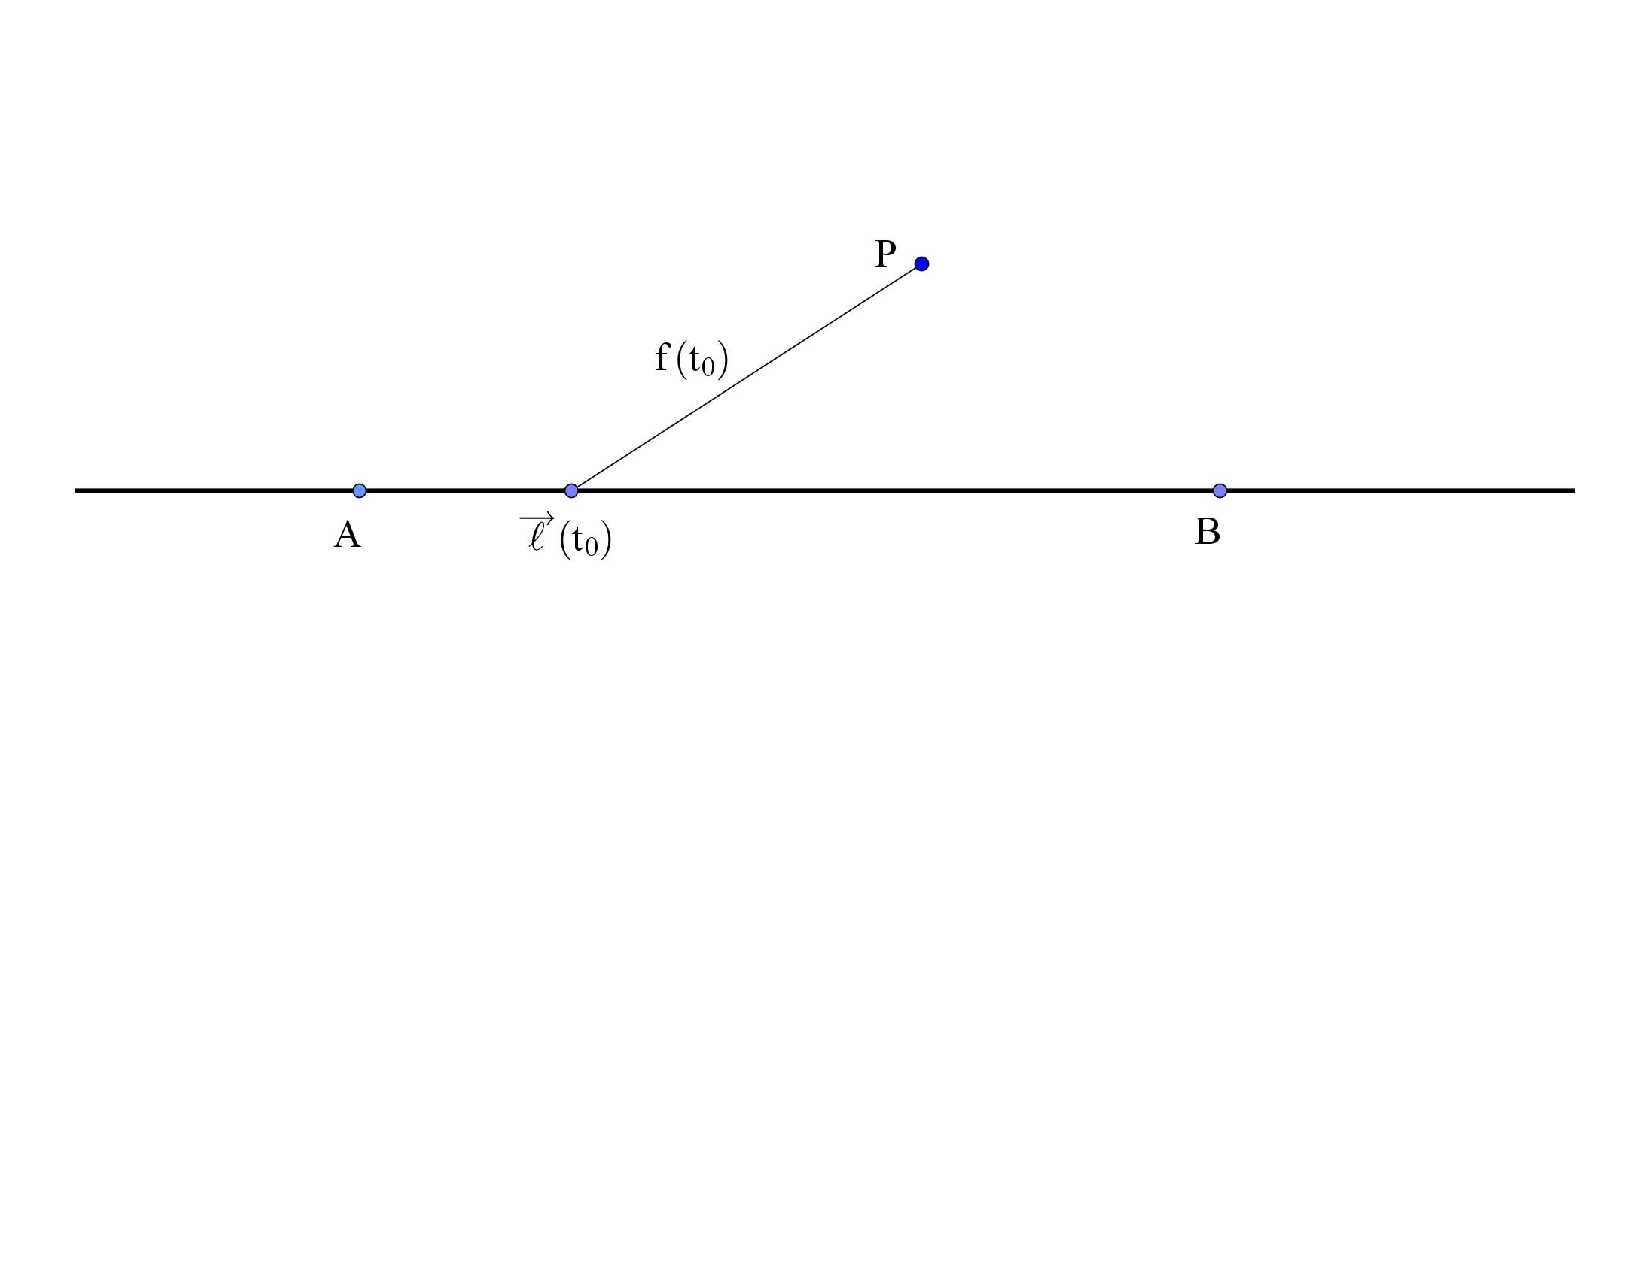
\includegraphics[scale=0.5]{distance.pdf}
\end{center}

\includegraphics[scale=0.5]{start.pdf}
{{{1\linewidth}{Your answer to this part depends on your parametric equations from part (a).  Using the parameterization given the distance from $P$ to an arbitrary point on line $L$ is given by $f(t)=\sqrt{(4-t)^2+(3-3t)^2+1}$.}}}
\includegraphics[scale=0.5]{end.pdf}


\item The distance from the point $P$ to line $L$ is the shortest distance.  Calculate the value of $t$ which minimizes the distance from the point $P$ to line $L$; that is, calculate the value of $t$ which minimizes $f(t)$ from part (b).

\begin{center}
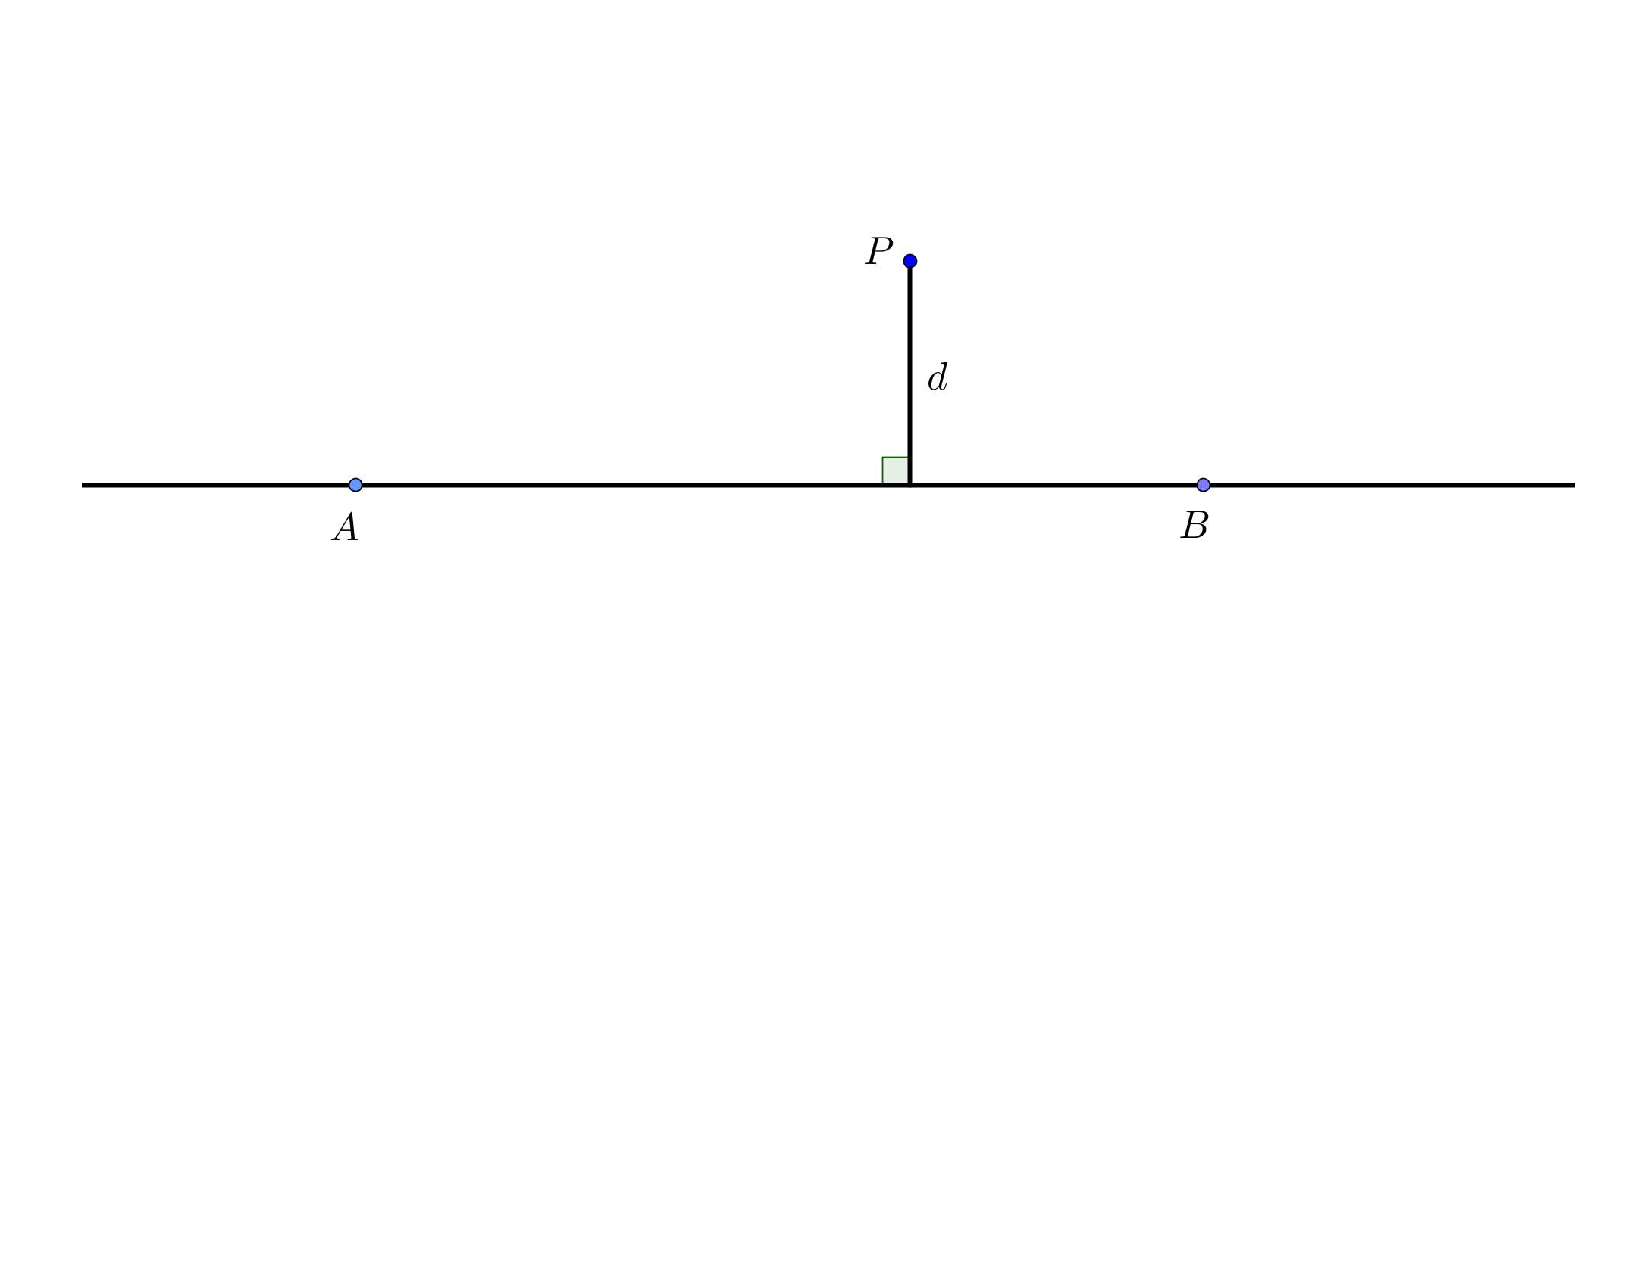
\includegraphics[scale=0.5]{length.pdf}
\end{center}

\includegraphics[scale=0.5]{start.pdf}
{{$t=\frac{13}{10}$; again, this depends on your parameterization of the line.}}
\includegraphics[scale=0.5]{end.pdf}


\item Compute the distance from the point $P(5,3,0)$ to line $L$ by calculating the distance from this $P$ to the point on your the line which corresponds to your value of $t$ from part (c).  Verify your answer with HW 11.3 \#10(b).

\includegraphics[scale=0.5]{start.pdf}
{{$d=\sqrt{\frac{91}{10}}$}}
\includegraphics[scale=0.5]{end.pdf}


\end{enumerate}


\end{enumerate}

\end{document}